\underline{LDA - \textit{Linear discriminant analysis}} jest używana do znalezienia liniowej kombinacji cech, które najlepiej rozróżniają dwie lub więcej klas obiektów lub zdarzeń. Wynikowe kombinacje są używane jako klasyfikator liniowy lub, częściej, służą redukcji wymiarów do późniejszej klasyfikacji statystycznej. 

Rozważmy zbiór obiektów z których każdy jest opisywany przez wektor cech \textbf{x}, przy czym dla każdego obiektu znana jest jego przynależność do klasy y. Podejście LDA bazuje na założeniu, że funkcje gęstości prawdopodobieństwa $ \forall i \rightarrow p(\textbf{x}|y = i) $ mają rozkłady normalne i jednakowe macierze kowariancji:

$ S = \dfrac{1}{n-1} \sum\limits_{i=1}^{i=n}(x_i - \bar{x})(x_i - \bar{x})^{T} $

LDA próbuje znaleźć podprzestrzeń cech, która maksymalizuje separowalność klas. Dla przypadku dwóch klas oraz dwuwymiarowego wektora cech szukamy takiego kierunku, dla którego rozkłady rzutów zbiorów poszczególnych klas na ten kierunek są jak najbardziej rozdzielone od siebie (rys.~\ref{lda}).

\begin{figure} [H]
	\centering
	\begin{subfigure}{.99\textwidth}
		\centering
		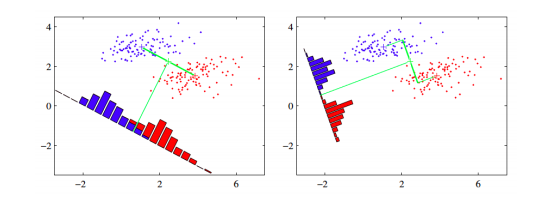
\includegraphics[width=1.0\linewidth]{EDMIIssues/Figures/lda.png}
	\end{subfigure}
	\caption{Przykład LDA.}
	\label{lda}
\end{figure}

\underline{QDA - \textit{Quadratic discriminant analysis}} - zakładamy różne macierze kowarjancji. QDA również próbuje znaleźć podprzestrzeń cech, która maksymalizuje separowalność klas. Dla powyszego przypadku będzie szukać najlepszego rzutu dla rozszerzonego dwuwymiarowego wektora cech o wartości 2-go rzędu tzn. $ [x_1, x_2] \rightarrow [x_1, x_2, x_1^2, x_1x_2, x_2^2] $.

\underline{PCA - Principal components analysis}

\begin{itemize}
	\item zakładamy zbiór wielowymiarowych obserwacji, leżących w przestrzeni $ R^p $,
	\item najczęsciej  obserwacje  nie są  równomiernie  rozrzucone wzdłuż wszystkich kierunków układu współrzędnych,
	\item koncentruj się w pewnych podprzestrzeniach przestrzeni $ R^p $,
	\item kierunki, wzdłuż których znajduje się większość obserwacji, nie muszą się pokrywać z osiami układu współrzędnych $ R^p $,
	\item próba losowa pochodzi z populacji o ciągłym rozkładzie w przestrzeni $ R^p $ z wektorem wartości oczekiwanych \textbf{m} i macierzą kowarjancji \textbf{S}
\end{itemize}

Pierwszą składową główną szukamy poprzez znalezienie takiego kierunku $ \gamma_1 \in R^p $, aby rzut ortogonalny wektora losowego \textbf{x} na ten kierunek dawał zmienną losową o największej warjancji. Kolejne składowe szukamy w ten sam sposób biorąc pod uwagę warunek aby kolejne kierunki były prostopadłe do poprzednich.

Pierwszą składową główną wektora \textbf{x} nazywamy rzut tego wektora na znaleziony kierunek przesunięty o wartość średnią:

$ y_1 = \gamma_1^T(\textbf{x} - \textbf{m}) $

Kolejne składowe główne odpowiadają kolejnym wektorom własnym macierzy kowarjancji \textbf{S}. Pierwsza składowa główna odpowiada wektorowi własnemu o największej wartości własnej ($ \lambda_1 $), kolejne wektory -> kolejne największe wartości własne.

Wielkość:\newline
$ \dfrac{\lambda_1 + ... + \lambda_k}{\lambda_1 + ... + \lambda_p} $\newline
wyraża procent zmienności wektora losowego $ x $ wyjaśnionych przez $ k $ ($ k \le p $) pierwszych składowych głównych.

\underline{Skalowanie wielowymiarowe}

Niech $ d_{ij} $, $ i $, $ j = 1, ..., n $ będą odległościami euklidesowymi między obserwacjami $ \textbf{x}_i $  oraz $ \textbf{x}_j $ w przestrzeni $ R^p $. Zadanie polega na znalezienie takie podprzestrzeni $ R^r $ o wymiarze $ r $, by odległości euklidesowe $ d_{ij}' $ mięszy rzutami obserwacji na tę podprzestrzeń minimalizwowały sumę\newline $ V = \sum\limits_{i=1}^n \sum\limits_{j=1}^n ({d_{ij}}^2 - {d_{ij}'}^2) $

Podobienstwo pomiędzy skalowaniem  wielowymiarowym  ,a  analizą  składowych głównych staje się równoważnością, gdy dana macierz $ d_{ij} $ jest macierzą odległości euklidesowych.

\underline{Autoencoder} - jest rodzajem sztucznej sieci neuronowej wykorzystywanej do uczenia się wydajnego kodowania danych w sposób nienadzorowany. Celem \textit{autoencodera} jest nauczenie się reprezentacji (kodowania) zestawu danych, zazwyczaj w celu zmniejszenia wymiarów, poprzez szkolenie sieci w zakresie ignorowania „szumu” sygnału.

\textbf{Przykład}

Powiedzmy że reprezentujemy zdanie poprzez wektor o długości liczby słów występujących w słowniku. Jeśli słowo występuję w zdaniu, wartość elementu wektora odpowiadającego temu słowu wynosi 1, jeśli słowo występuje dwukrotnie - 2 itd... Słowniki składają się z tysięcy słów, więc nieoptymalna jest reprezentacja zdania w takiej przestrzeni, ponieważ tylko ułamek procenta składowych wektora reprezentującego jakiekolwiek zdanie będzie niezerowych. 

Aby uzyskać reprezentację zdania w mniejszej przestrzeni możemy użyc \textit{autoencodera}. Nasz zbiór uczący przepuszamy przez sieć neuronową gdzie warstwa wejściowa składa się z $ N $(ilość słów w słowniku) neuronów. Warstwa wyjściowa również składa się z $ N $ neuronów. Pomiędzy tymi warstwami jest nieparzysta liczba warstw ukrytych (zazwyczaj symetrycznych), a środkowa warstwa reprezentuje wektor kodujący (rys.~\ref{autoencoder}). Podczas uczenia na wyjściu ustawiamy ten sam wektor co na wejściu.

\begin{figure} [H]
	\centering
	\begin{subfigure}{.99\textwidth}
		\centering
		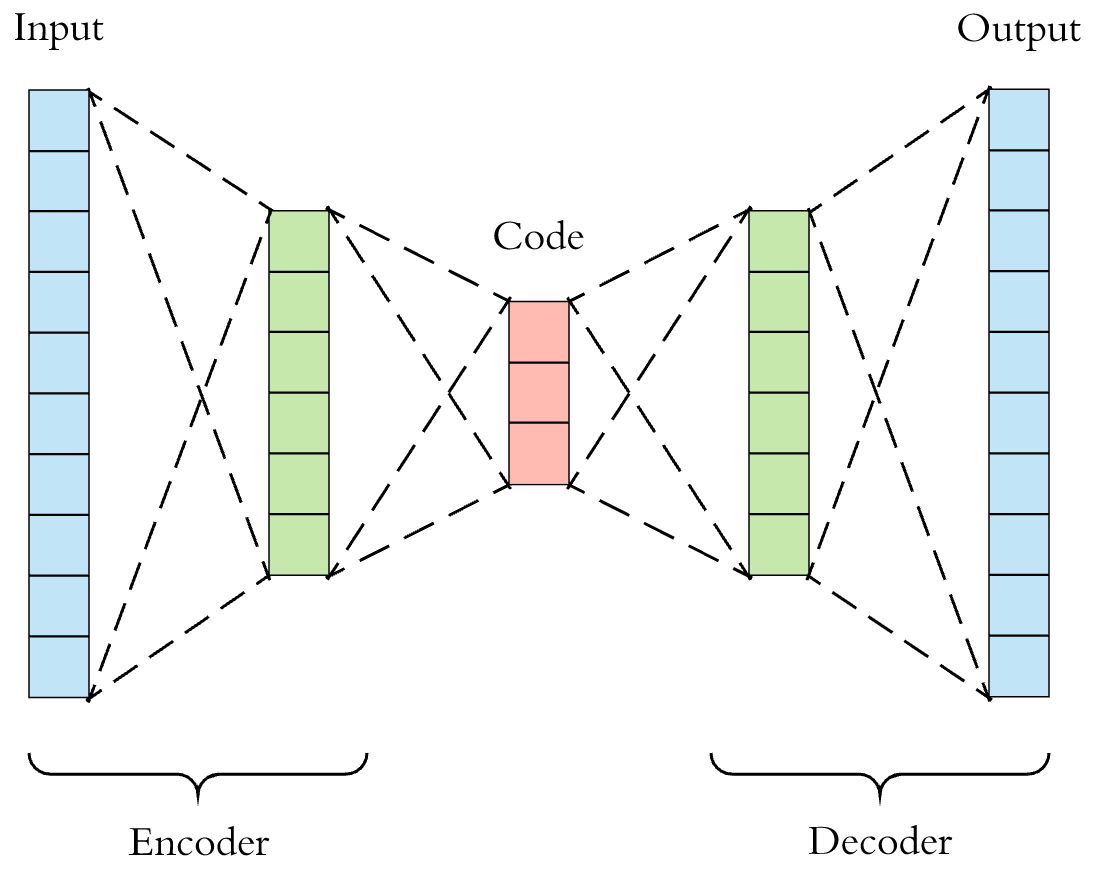
\includegraphics[width=1.0\linewidth]{EDMIIssues/Figures/autoencoder.png}
	\end{subfigure}
	\caption{Topologia sieci neuronowej typu \textit{autoencoder}.}
	\label{autoencoder}
\end{figure}